\section{Response to Questions on Lab 1}

Several questions were raised in the lab 1 report. The following is a response to those questions.

\vspace{1em}
\textit{1. The detail of the failed circumnavigation attempt.}
\vspace{1em}

\textbf{Answer 1}: 
During an attempt at becoming the first woman to complete a 
circumnavigational flight of the globe in 1937 in a Purdue-funded 
Lockheed Model 10-E Electra, Earhart and navigator Fred Noonan 
disappeared over the central Pacific Ocean near Howland Island. 
The two were last seen in Lae, New Guinea, on July 2, 1937, on the 
last land stop before Howland Island and one of their final legs of the flight. 
She presumably died in the Pacific during the circumnavigation.
Nearly one year and six months after she and Noonan disappeared, Earhart was officially declared dead. 

\begin{figure}[!htp]
    \centering
    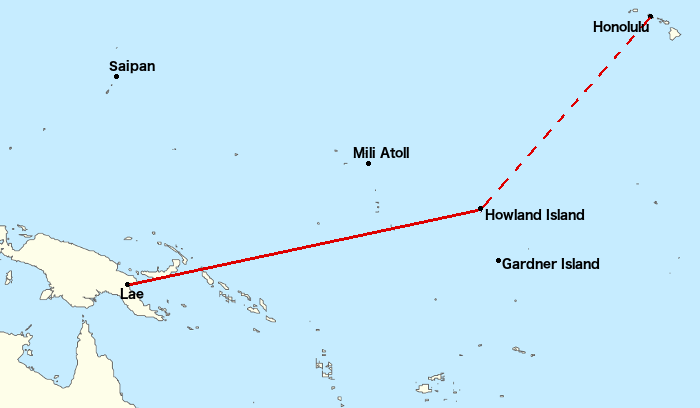
\includegraphics[width=0.9\textwidth]{images/Earhart_locations.png}
    \caption{Earhart's last flight path (red) superimposed on a map of the Pacific Ocean. Dashed line indicates the last presumed course from Howland Island.}
\end{figure}

Many researchers believe that Earhart and Noonan ran out of fuel while searching for Howland Island, ditched at sea, and died.
At 6:14 AM Itasca time, Earhart estimated they were 200 mi (320 km) away from Howland. As the plane closed with the island, it expected to be in radio contact with Itasca. With the radio contact, the plane should have been able to use radio direction finding (RDF) to head directly for the Itasca and Howland. The plane was not receiving a radio signal from Itasca, so it would have been unable to determine a respective RDF bearing. Although Itasca was receiving HF radio signals from the plane, it did not have HF RDF equipment, so it could not determine a bearing to the plane. Almost no communications were transmitted to the plane. Consequently, the plane was not directed to Howland, and was left on its own with little fuel.
It is widely believed that the plane eventually ended up very close north of Howland Island, or on the way
turning to the south to look for the other island, known as Gardner Island (now Nikumaroro).


\vspace{1em}
\textit{2. Why the design failed?}
\vspace{1em}

\textbf{Answer 2}:
One of the factors that contributed to the decline of the Model 10 Electra was the introduction of newer, faster, and more efficient aircraft designs. As commercial air travel became more popular, airlines sought planes that could transport passengers more quickly and at a lower cost. The Electra was considered outdated compared to newer planes like the Douglas DC-3, which offered more space, comfort, and speed.

Another issue with the Model 10 Electra was that it had a reputation for being difficult to handle. The aircraft was known for being heavy and hard to maneuver, which made it challenging for pilots to fly in certain conditions. This reputation was further cemented by the tragic disappearance of Amelia Earhart and her Electra.